\documentclass[12pt, openany]{book}

\usepackage{color}
\usepackage[english]{babel}
\usepackage[utf8]{inputenc}
\usepackage{indentfirst}
\usepackage{graphicx}
\usepackage{verbatim}
\usepackage{listings}
\usepackage{url}
\usepackage{stringenc}
\usepackage{pdfescape}
\usepackage{subfig}
\usepackage{float}
\usepackage{eurosym}
\usepackage[toc,page]{appendix}
\usepackage{geometry}
\geometry{a4paper, total={160mm,240mm}, left=25mm, top=25mm}
\makeatletter
\def\@makechapterhead#1{%
  \vspace*{50\p@}%
  {\parindent \z@ \raggedright \normalfont
    \ifnum \c@secnumdepth >\m@ne
      \if@mainmatter
        %\huge\bfseries \@chapapp\space \thechapter
        \Huge\bfseries \thechapter.\space%
        %\par\nobreak
        %\vskip 20\p@
      \fi
    \fi
    \interlinepenalty\@M
    \Huge \bfseries #1\par\nobreak
    \vskip 40\p@
  }}
\makeatother
\usepackage{xspace}

\begin{document}

\newcommand{\drugbank}{\texttt{DrugBank}\xspace}
\newcommand{\alephilp}{\texttt{Aleph}\xspace}
\newcommand{\wordvec}{\texttt{Word2Vec}\xspace}
\newcommand{\python}{\texttt{Python}\xspace}
\newcommand{\prolog}{\texttt{Prolog}\xspace}
\newcommand{\swi}{\texttt{SWI-Prolog}\xspace}
\newcommand{\yap}{\texttt{YAP}\xspace}
\newcommand{\xml}{\texttt{XML}\xspace}
\newcommand{\tensorflow}{\texttt{TensorFlow}\xspace}
\newcommand{\numpy}{\texttt{NumPy}\xspace}



\title{\Huge{\textbf{\textit{DrugBank Data Mining}}}\linebreak
\Large\textbf{\\Prediction of Drug Interactions using \linebreak Inductive Logic Programming \linebreak and Neural Networks}
\linebreak\linebreak\linebreak

\includegraphics[width=8cm]{feup.pdf}\linebreak \linebreak
\large{MIEIC} \linebreak
\large{Programming Paradigms}\linebreak
}
\author{
Ângela Filipa Pereira Cardoso - 200204375 (angela.cardoso@fe.up.pt)\\
\\
\\ Faculdade de Engenharia da Universidade do Porto \\ Rua Roberto Frias, 4200-465 Porto, Portugal
 \vspace{1cm}}
\maketitle
\thispagestyle{empty}

%************************************************************************************************
%************************************************************************************************
 
\chapter*{Abstract} 
The aim of this work is to predict drug interactions in the Canadian drug database \drugbank. The fact that this database has both structured and unstructured information, compelled us to use two different learning tools. We use the Inductive Logic Programming tool \alephilp, on the categorical fields. For the free text, we use the Neural Network \wordvec. We will show that, although initial results where encouraging and showed a slight improvement when \wordvec data was included, the final tests are extremely disappointing and there is no improvement from the \wordvec data. 


\tableofcontents

%************************************************************************************************
%************************************************************************************************

%*************************************************************************************************
%************************************************************************************************



\chapter{Introduction}

This work is part of an ongoing post doctoral research scholarship from the project NanoStima, within the research center CRACS from INESC TEC. It is joint work with Rui Camacho, In\^es Dutra and V\'itor Santos Costa.

\drugbank is an extensive Canadian drug database, containing semistructured information. The database format is \xml and there are some categorical and some free text fields. As a part of the database, there is a classification of all the previously identified drug to drug interactions. For each drug there is a list of drugs with which there is some interaction, as well as a description of the type of interaction. Our main objective is to predict these interactions from the other information present in this dataset and maybe elsewhere. If successful we may extend our work to predict interactions by type, which should be extracted from the descriptive text of each interaction. Also, if we devise a method that does a good job of predicting drug interactions, any predicted interactions that are not in the database may be real interactions that are yet to be realized.

\wordvec is a Neural Network, developed by Mikolov et al, that given a natural language text, transforms each word of the language into a vector in a high dimensional space, in such a way that words with similar contexts in the text are represented close to each other in the vector space. By context we understand the words surrounding (at a predefined distance) our objective word whenever it appears in the text. Our idea is that drugs with similar contexts should have some relation. In such a way that for example if drugs A and B are represented very close together in the vector space and drug A interacts with drug C, perhaps drug B also interacts with drug C.

\alephilp (A Learning Engine for Proposing Hypotheses) is an Inductive Logic Programming system developed by Ashwin Srinivasan with input from several others. There are three files in an \alephilp program: the background file, containing all the knowledge about our data; the positive examples file, which contains the examples we want to predict; and the negative examples file, which contains examples that are not supposed to be predicted by our theory. The basic \alephilp procedure can be described in 4 steps:
\begin{itemize}
	\item Select an example to be generalized.
	\item Construct the most specific clause that entails the example selected, and is within language restrictions provided, the ``bottom clause''.
	\item Find a clause more general than the bottom clause. This is done by searching for some subset of the literals in the bottom clause that has the ``best'' score.
	\item The clause with the best score is added to the current theory, and all examples made redundant are removed. 
\end{itemize}

Our idea was to use \alephilp for the structured part of \drugbank, while extracting information from the free text portion using \wordvec.

\chapter{System Description}
\section{Conceptual Description}
\subsection{Functionalities}

The main purpose of the system is to train and test drug interactions using \alephilp on the \drugbank database. For that there are several components and each has its own functionality:
\begin{itemize}
	\item The \texttt{drugbank.py} module allows the user to prepare parts of the \xml to be used with the \wordvec software or with \alephilp. It has several modes, namely:
	\begin{itemize}
		\item \texttt{hyphens} - replaces the hyphens in the tags of an \xml file with underscores, so that they will not interfere with \prolog's interpretation of hyphens;
		\item \texttt{names} - creates a file with the names of the selected drugs in \texttt{drugbank.xml} and another file with the same names concatenated, so that they can be seen as single words by \wordvec;
 		\item \texttt{word2vec} - extracts the free text from the selected drugs in \texttt{drugbank.xml}, preparing it for \wordvec to do its analysis;
		\item \texttt{prolog} - extracts the parts of the selected drugs in \texttt{drugbank.xml} that are appropriate for introducing in \alephilp, that is, the mostly categorical and structured tags, whose information is considered pertinent to the task.
	\end{itemize}
	\item The \texttt{word2vec.py} module is used to turn the text obtained from \texttt{drugbank.py} into an array of vectors, each representing a word in the text. Several things can be configured in order to obtain the best results, such as the number of words that are considered part of the context of each word, the type of neural network to be used (\texttt{CBOW} or \texttt{Skip-Gram}), the number of steps of the network and the size of the vector space to use for the embeddings.
	\item The \texttt{filter.py} module filters \wordvec data, selecting the words that belong to a provided list. We use it to consider only drug names in our final analysis.
	\item The \texttt{linkage.py} module is used to compute a hierarchical clustering of the word vectors produced by \wordvec.
	\item The \texttt{cophenet.py} module is used to compute the cophenetic correlation coefficient of the clustering computed by \texttt{linkage.py}. This metric is used as a quality measure for the clustering process.
	\item The \texttt{word2vec-filter-500.ipynb} \texttt{Jupyter} \texttt{Notebook} was used to extract the actual clusters of words to be used in \alephilp. They also allow us to visualize the Hierarchical Clustering.
	\item The \texttt{word2vec.pl} module transforms the clusters obtained from the \texttt{Jupyter} \texttt{Notebook}s into \prolog facts.
	\item The \texttt{drugbank.pl} module parses the \xml file obtained from the \texttt{drugbank.py prolog} module into \alephilp background, and positive and negative examples files.
	\item The \texttt{drugbank\_test.pl} module is very similar to the previous one but was specifically designed to create sets of experiences in which one can train and test both with or without the \wordvec clusters.
\end{itemize}

\subsection{Architecture}
	
Since the system modules and their functions have been described in the previous section, we present here, in Figure~\ref{diagram}, the component diagram, with the interactions showing the intended order of use of each module. In other words, the arrows represent information flow from one component to the next.

\begin{figure}[ht]
\begin{center}
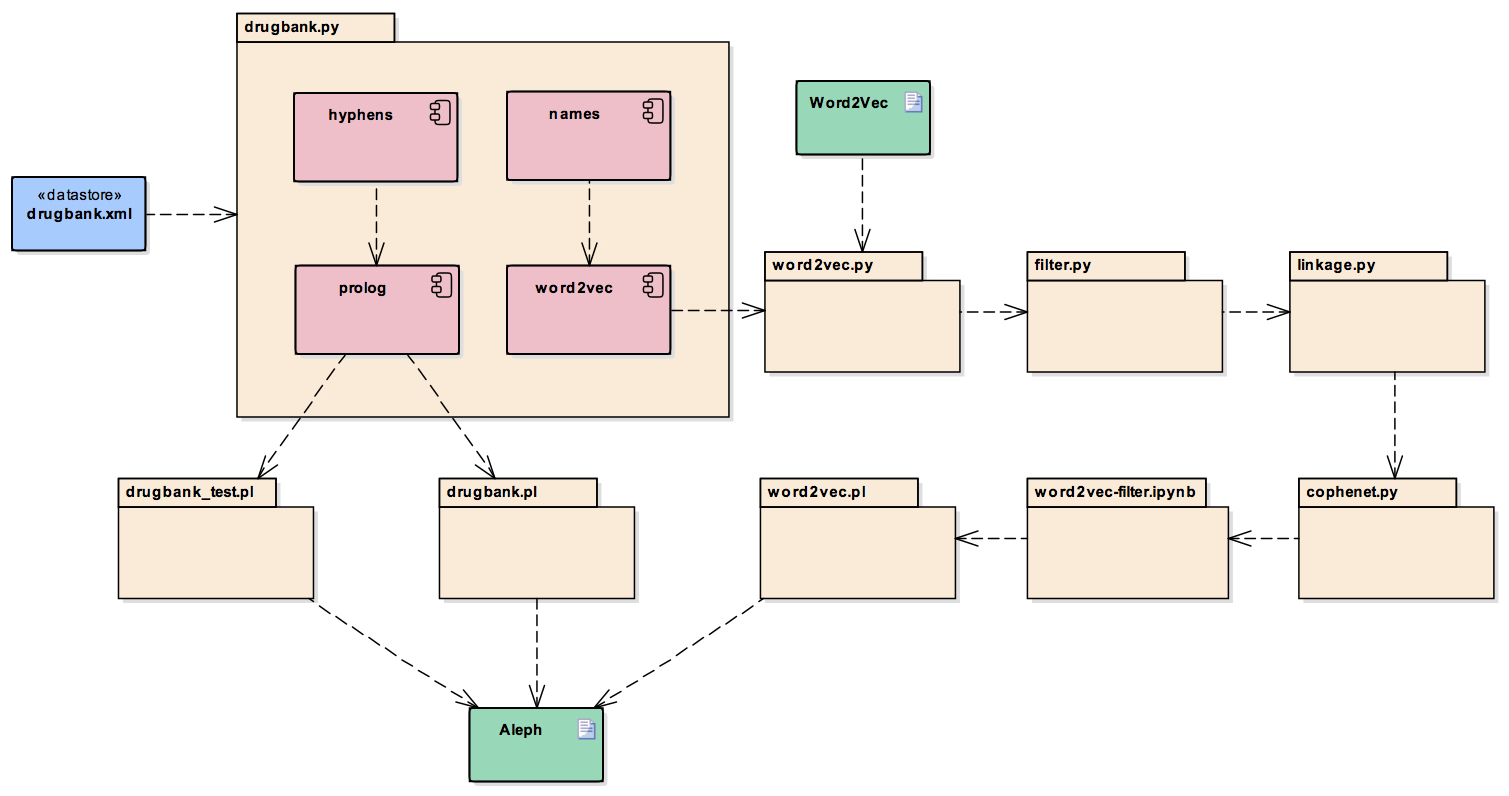
\includegraphics[width=16cm]{diagram.jpg}
\caption{Component diagram with interactions}
\label{diagram}
\end{center}
\end{figure}

\subsection{Programming Languages}

\subsubsection{Python}

The first programming language chosen was \python. As seen in the description of the modules, we use it to work with the \xml file, preparing it for \prolog and extracting text portions for \wordvec. It is also used to compute the word clusters that will be used in the final step as extra information for \alephilp. 

The main reason that lead to this choice was the fact that \wordvec, as a part of the \tensorflow library, is available in \python. Also, \python is a language widely used by scientists, so it fits very well with this project, given its scientific nature. There are uncountable \python libraries and tutorials for all kinds of scientific purposes, which made this work much easier. 

\python is a multi-paradigm programming language, depending on the use, it can be object-oriented, imperative, functional, procedural or reflective. As used in this application it was mostly procedural, because there was no real need for the structure of an object oriented approach. Also, the examples found online similar to our purpose where procedural.

Examples of other procedural programming languages are \texttt{Fortran}, \texttt{ALGOL}, \texttt{COBOL}, \texttt{BASIC}, \texttt{Pascal}, \texttt{C}, \texttt{Ada} and \texttt{Go}. The first of these are outdated and do not make very good choices. \texttt{C} is still very current and \texttt{Go} is actually quite new. With \texttt{C} one gets the advantage of having a faster application, at least assuming a good coding skill. In fact, since \python is interpreted instead of compiled, \texttt{C} can be much faster. However, it is harder to write \texttt{C} code and it is much less supported for our intended purpose. Of course speed can be an issue, as we will see in the discussion of the results, but in our case, the problem is in \alephilp and not in \python, which can handle the necessary data in a timely fashion. As for \texttt{Go}, it is far to young to have any kind of libraries that would facilitate our work, we would have to build everything from scratch, so it made no sense to choose it. 

\subsubsection{Prolog}

The choice of \prolog was mandatory once the decision to use Inductive Logic Programming as a learning tool was made. There are many other learning methods, but this one provides a theory that can be used as an explanation of the model it proposes. In this case, since we are trying to predict drug interactions, a theory could tell us the conditions that lead to drugs interacting with each other. This kind of explanation can be very useful in medical, financial and other settings, where even when the model guesses correctly, people still want to understand why.

There are several flavors of \prolog and we use two. The first one is \yap, which is used to run \alephilp. This was also a very clear choice, since \alephilp was made for \yap, where it has the most support and runs faster. However, to prepare the files for \alephilp (in the modules word2vec.pl, drugbank.pl and drugbank\_test.pl) we decided to use \swi. There where two reasons for this. First, \swi is very well documented and has several libraries that make certain tasks (such as importing \xml files) much easier. Second, in their current versions \swi is much more stable than \yap.

As far as we know, there are no alternatives to \prolog for Inductive Logic Programming, so the choice was just on which implementation of \prolog to use. The two used and considered seem the best for their respective jobs. Also, since they are both open source, they where preferred over others such as \texttt{SICStus} \prolog.

\subsection{Other Applications}

\subsubsection{Python}

As we discussed above there are many scientific applications of \python. The main libraries used by these applications are:
\begin{itemize}
\item \numpy \xspace - a low level library written in \texttt{C} and \texttt{Fortran} for high level mathematical functions (so it does not really count as a \python written application).
\item \texttt{SciPy} - a library that uses \numpy for more mathematical functions and comes with modules for various commonly used tasks in scientific programming, including linear algebra, integration (calculus), ordinary differential equation solving and signal processing.
\item \texttt{Matplotlib} - a flexible plotting library for creating interactive 2D and 3D plots that can also be saved as manuscript-quality figures.
\item \texttt{Pandas} - a data manipulation library based on \numpy which provides many useful functions for accessing, indexing, merging and grouping data easily.
\item \texttt{Rpy2} - a \python binding for the \texttt{R} statistical package allowing the execution of \texttt{R} functions from \python.
\item \texttt{PsychoPy} - a library for cognitive scientists allowing the creation of cognitive psychology and neuroscience experiments.
\item \tensorflow \xspace - an open source software library for numerical computation using data flow graphs.
\end{itemize}

The main thing relating these applications to ours (in addition to the fact that we make use of many of them) is the fact that each one of them provides a set of tools to deal with common scientific programming needs.

\subsubsection{Prolog}

There are several uses of \prolog and \alephilp in the setting of data mining. For concrete examples, one can see the scientific publications of Rui Camacho, In\^{e}s Dutra and V\'{i}tor Santos Costa, among others. These where the works that inspired the use of \alephilp in this setting, so the similarity is obvious, although the results are quite less attractive.

\section{Implementation}
\subsection{Implementation Details}

The \python modules are essentially a collection of tools to perform several tasks. The original input is an \xml file with a fixed structure. As for the output, it can be a redacted version of the \xml file, a \numpy array or a \texttt{Pickle} file. The \texttt{Pickle} files and \numpy arrays are used as input from one \python module to another. The redacted \xml is used by the \prolog modules. In this sense, there is no specially structured communication method between the \python and the \prolog parts. Since they can both process \xml and the original data is in that format, that is the format used to pass data from one to the other.

\subsection{Development Environment}

We used \texttt{PyCharm} as the main development environment for \python. \texttt{Jupyter Notebook} was also wildly used, not just for its final task of extracting the clusters and showing the hierarchical clustering diagram, but also as a way to quickly test some \python code.

As for \prolog, we decided to use the text editor \texttt{Sublime Text} with a specific \prolog plugin.

The terminal application chosen was \texttt{iTerm 2}.

A portable computer running \texttt{macOS Sierra} is where the code was written and some faster parts where tested and run. A virtual machine, provided by INESC TEC, with 240GB of memory, 16 cores and running \texttt{CentOS} was used to run \alephilp and some \python modules that where slower, such as \texttt{word2vec.py}, \texttt{linkage.py} and \texttt{cophenet.py}b, when there was a lot of data to process.

\chapter{Results}

Our first test was done using the first 100 drugs from \drugbank and the interactions they have with each other. In this test, \wordvec usage improved the recall in about 5\%, so we where encouraged. It was also clear from this test that 100 was about the number of drugs we could use in each test in order for \alephilp to finish its task in a timely manner. In fact, using \wordvec data, \alephilp can take up to a day to finish, depending on the amount of information of the drugs.

In order to test our learning method, we used a set containing the first 500 drugs on the database. For that set, we performed 10 tests. In each test, we randomly selected 100 drugs for training and used the rest for testing. The drug to drug interactions considered are only the ones among each group. And for the negative examples we took about 10 times as much as the positives.

The results are detailed in the file \texttt{accuracy\_precision\_recall.xlsx} provided with this report. In Figure~\ref{chart} we can observe a the precision recall curves for our training and test sets. For each set, we used two methods, one with only \alephilp and another with \alephilp and \wordvec.

\begin{figure}[ht]
\begin{center}
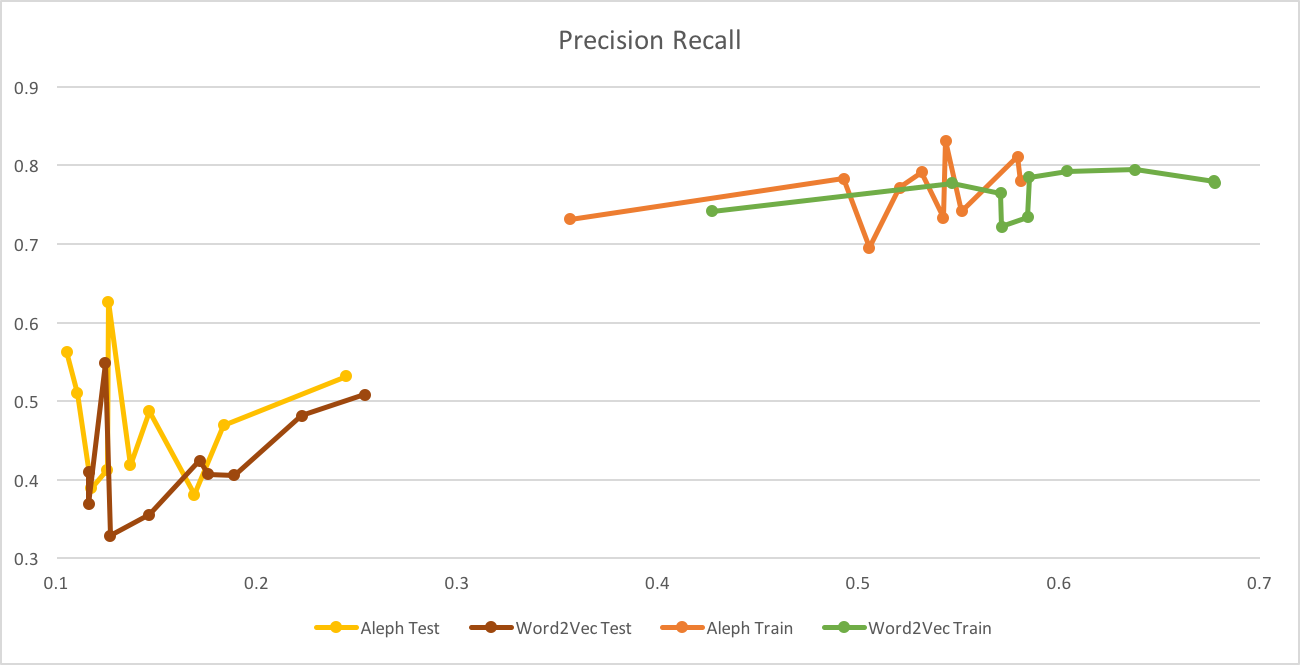
\includegraphics[width=15cm]{chart.png}
\caption{Precision recall curves}
\label{chart}
\end{center}
\end{figure}

One can observe that although the training results are good, the models fail on all tests. Also, there is no significant difference in quality of the results between using \wordvec data or not. However, when provided with \wordvec data, \alephilp does choose to use it in its theories quite often. This can be checked in the files \texttt{drugbank\_all\_500\_N.pl}, where \texttt{N} is the test number, between 1 and 10.

\chapter{Conclusion}

The results from our preliminary tests are very discouraging. In fact, our method fails to predict drug interactions in a satisfactory way. However, this was an important learning experience and it is our hope to be able to improve this method and its results.

It is quite clear that there is much to be gained from using different languages to do different parts of an application. Also, depending on the application different paradigms may be very useful and are one of the main reasons to use more than one language.

\chapter{Improvements}

This is very much a work in progress so there are plenty of improvements to be made. The code itself can be better organized, although it is quite better now than when the first experiments began. The main improvements though should be made in the method. For this we have several ideas, such as:
\begin{itemize}
	\item Use a clustering method to obtain groups of drugs where \alephilp can be used with more success, since \alephilp is proposing a very large theory with each rule covering only some examples.
	\item Use other data such as molecular describers for the drugs or patient drug usage and effects reports.
	\item Change the way we are using \wordvec in order to obtain better information from it, for example, use a different context size, a different clustering method or no clustering at all using only a maximum distance between word vectors.
	\item Change the settings in \alephilp or the modes and determinations used.
	\item Try other parts of the \xml in \alephilp.
\end{itemize}
It is our hope that these and other ideas will lead to a good method for predicting drug interactions.

\chapter{Resources}
\section{Bibliography}
\subsection{Publications}
\begin{description}
\item Distributed Representations of Words and Phrases and their Compositionality; Tomas Mikolov, Ilya Sutskever, Kai Chen, Greg Corrado and Jeffrey Dean; \url{http://papers.nips.cc/paper/5021-distributed-representations-of-words-and-phrases-}\linebreak\url{and-their-compositionality.pdf}.
\item Demand-Driven Clustering in Relational Domains for Predicting Adverse Drug Events; Jesse Davis, V\'itor Santos Costa, Peggy Peissig, Michael Caldwell, Elizabeth Berg and David Page; \url{http://icml.cc/2012/papers/644.pdf}.

\end{description}
\subsection{URLs}
\begin{description}
\item The Hitchhiker's Guide to Python - Scientific Applications, \url{http://docs.python-guide.org/en/latest/scenarios/scientific/}.
\item TensorFlow - Vector Representations of Words, \url{https://www.tensorflow.org/tutorials/word2vec}.
\item The Aleph Manual, \url{http://www.cs.ox.ac.uk/activities/machinelearning/Aleph/aleph.html}.
\item SciPy Hierarchical Clustering and Dendrogram Tutorial, \url{https://joernhees.de/blog/2015/08/26/scipy-hierarchical-clustering-and-dendrogram-tutorial/}.
\item Word2Vec Tutorial - The Skip-Gram Model, \url{http://mccormickml.com/2016/04/19/word2vec-tutorial-the-skip-gram-model/}.
\item Zichen Wang - TensorFlow Playground, \url{https://github.com/wangz10/tensorflow-playground/blob/master/word2vec.py#L105}.
\end{description}
\section{Software}
\begin{description}
\item PyCharm, JetBrains, \url{https://www.jetbrains.com/pycharm/specials/pycharm/pycharm.html}.
\item iTerm 2, George Nachman, \url{https://iterm2.com}.
\item Sublime Text, Sublime, \url{http://www.sublimetext.com}.
\item TensorFlow, \url{https://www.tensorflow.org}.
\item Aleph, \url{http://www.cs.ox.ac.uk/activities/machinelearning/Aleph/aleph}.
\end{description}


\begin{appendices}
\chapter{User Manual}

\begin{enumerate}
	\item Before using this software it is necessary to install some python packages. This can be done using pip. We recommend the usage of Python 3, since that was the tested version. Depending on your system, some packages may already be installed, so we will not list all of them. In any case, when calling any of the python modules, if a Python library is missing, it will say so and you can install it at that time.

	\item Install TensorFlow, following the instructions in \url{https://www.tensorflow.org/install/}.

	\item Execute \texttt{python3 drugbank.py word2vec N MODE [TYPES] \&}, where \texttt{N} is the number of drugs (0 if all); \texttt{MODE} is either `all' (for all types of drugs), `only' for drugs with all types in the list TYPES or some for drugs with at least one type in the list \texttt{TYPES}; and \texttt{TYPES} is a list of drug types, a subset of `approved', `illicit', `experimental', `withdrawn', `nutraceutical', `investigational' and `vet\_approved'.

	\item Execute \texttt{python3 drugbank.py names drugbank\_MODE[\_TYPES\_N].xml \&}, where \texttt{MODE}, \texttt{TYPES} and \texttt{N} are as above.

	\item Execute \texttt{python3 word2vec.py NAME DIMENSION DIAMETER RAY METHOD M \&}, where \texttt{NAME} is the word file name after \texttt{drugbank\_}, that is, \texttt{MODE[\_TYPES\_N]}; \texttt{DIMENSION} is the dimension of the embedding vector space, \texttt{DIAMETER} is the full size of the context of each word (in both directions); \texttt{RAY} is usually half of the \texttt{DIAMETER}; \texttt{METHOD} is either \texttt{skip-gram} or \texttt{cbow} and \texttt{M} is the number of steps to take when training the neural network.

	\item Execute \texttt{python3 filter.py MODE final\_embeddings\_NAME\_METHOD\_M\_DIAMETER\_RAY concatenated\_drug\_names\_NAME true}, with the parameters as above.

	\item Execute \texttt{python3 linkage.py final\_embeddings\_NAME\_METHOD\_M\_DIAMETER\_RAY\_}\linebreak\texttt{filter\_concatenated\_drug\_names\_NAME MODEL}, with parameters as above and \texttt{MODEL} the linkage model, for example `ward'.

	\item Execute \texttt{python3 cophenet.py final\_embeddings\_NAME\_METHOD\_M\_DIAMETER\_RAY\_}\linebreak\texttt{filter\_concatenated\_drug\_names\_NAME MODEL}, with parameters as above.

	\item Observe the files \texttt{word2vec.log} and \texttt{cophenet.log} to determine which embedding size is the best, it should be the one that converges in \wordvec and as the highest value of \texttt{cophenet}.

	\item Adapt the \texttt{Jupyter} \texttt{Notebook}  \texttt{word2vec-filter-500.ipynb} to your file names, in order to extract the actual clusters of words to be used in \alephilp.

	\item Copy the cluster list obtained in the previous step to the file \texttt{word2vec.pl} to generate the \wordvec \alephilp background; in \swi import the module \texttt{word2vec.pl} and run \texttt{word2vec\_2\_aleph.}; a file named \texttt{word2vec\_temp.pl} is generated; place it in the folder where you will run your experiments and rename it \texttt{word2vec.pl}.

	\item Execute \texttt{python3 drugbank.py prolog N MODE TYPES}, with the parameters as above.

	\item Execute \texttt{python3 drugbank.py hyphens drugbank\_NAME.xml}.

	\item In \swi import the module \texttt{drugbank\_test.pl} and run \linebreak 
	\texttt{xml\_2\_aleph('drugbank\_NAME.xml', TESTS, SIZE, TESTNAME).}, where \texttt{NAME} is as above, \texttt{TESTS} is the number of tests to generate, \texttt{SIZE} is the number of drugs to use in the training of each test set and \texttt{TESTNAME} is the base name for the test \alephilp files that will be generated.

	\item Copy the test files generated in the last step into two folders; change the background files (the ones with extension \texttt{.b}) in one of those folders to include the \texttt{word2vec.pl} file previously generated, by adding the line '\texttt{:- [word2vec].}'.

	\item Place the \texttt{aleph.pl} and \texttt{settings.yap} files supplied with this report in the test folders.

	\item In \yap run \hfill \hfill \linebreak
		\texttt{[aleph].}\linebreak
		\texttt{read\_all(TESTNAME\_I).}\linebreak
		\texttt{induce.}\linebreak
		where \texttt{TESTNAME} is as above and \texttt{I} is the number of the text (between 1 and \texttt{TESTS}, inclusively).
\end{enumerate}



\end{appendices}

\end{document}
